\chapter{Prototype Implementation}
\begin{chapterintro}
In this chapter we will describe the design and implementation of a prototype predictive module. This module is a software library which allows end users to actually obtain predictions using the knowledge we have acquired in previous stages of the project.

The prototype relies mainly on a \emph{Rule Engine}, which evaluates the input conditions (past events) and provides with predictions for the future. Further details on rule engines and the chosen implementation will be given as well.

Although the purpose of our prototype does not include user interfaces or any visualisation, we will provide examples on how an actual predictive interface can be presented to maintenance operators.
\end{chapterintro}

\label{chap:prototype}
\section{Module description}
\label{sec:module_description}
In this section we will provide a general description of the implemented prototype. This prototype allows the usage of already existing association rules, which have been already obtained as the result of a \emph{Data Mining}\cite{torgo2003data}\cite{han2006data} procedure. These rules do not offer any functionality by themselves, as a system is needed to check whether their conditions are fulfilled and therefore a prediction can be made.

Rules are simply textual information in the form of "When A and B happen together, C has 80\% chances of happening". This information would be useful for an operator who might be manually checking events and would be able to expect C after seeing A and B. However, real systems usually have a much larger set of possible events, and many more events happening during each observation, and therefore an automated system is needed to perform these operations.

We call such a system a \emph{Rule engine}\cite{liang2009openrulebench}. A rule engine is simply a system which evaluates input conditions and fires the rules which comply with these conditions, outputting the result of said rules. In our case, the system will take as input a set of current events, and output a list of predictions along with their probabilities.

The implementation of a rule engine is not a trivial matter, and requires a significant amount of work to achieve optimal results in terms of computation requirements and complexity. Therefore, we will count on one of the already existing solutions which suits our needs perfectly and in a very optimised way: the JBoss Drools Expert library\cite{browne2009jboss}. This library is freely available as a java module and counts on several interoperability options, which makes it perfect for the usage in our project. The only requirement this imposes is the need of translating our rules to a Drools-compatible format, a matter which will be addressed later on this document.

\subsection{Parameters and interfaces}
\label{sec:parameters_and_interfaces}
Depending on our needs for each situation, our system can obtain predictions for several periods of time, different types of systems and different input lengths. Specifically, we count on rules for four different stations of different characteristics (Stations A, B, C and D) and for three different time windows (one day, two days and seven days). Each of these prediction modes needs a different type of input and needs to use a different set of rules. This distinction has therefore been made at the time of generating the rules, and now those rules need to be loaded accordingly to the kind of prediction we want to obtain.

In other words, said parameters (station type and time window) fixes the set of rules to be used and the length of the input to be provided. This association also works in the other direction: by using an specific rule set and an specific input, we are already defining the execution parameters. Therefore, both the station type and prediction time window are irrelevant for the correct function of our predictive module. It is responsibility of the operator or executing system to select the appropriate rule set and provide an appropriate input. This allows new execution options to be added or updated at any time, without the need of modifying the module in any way. If we generate a new set of rules expecting a whole month of input and which will generate a month of predictions, we just need to load it and know what it is generating. Also, if we generate rules for a new type of maintenance station we just need to load them on the module and provide an input according to that new type of station.

The architecture of the module is very simple. It counts on an Engine class which streamlines the whole procedure, relying on three model classes to provide Alarm and prediction representations. A class diagram can be seen in figure~\ref{fig:prototypeArchitecture}

\begin{figure}[hbtp]
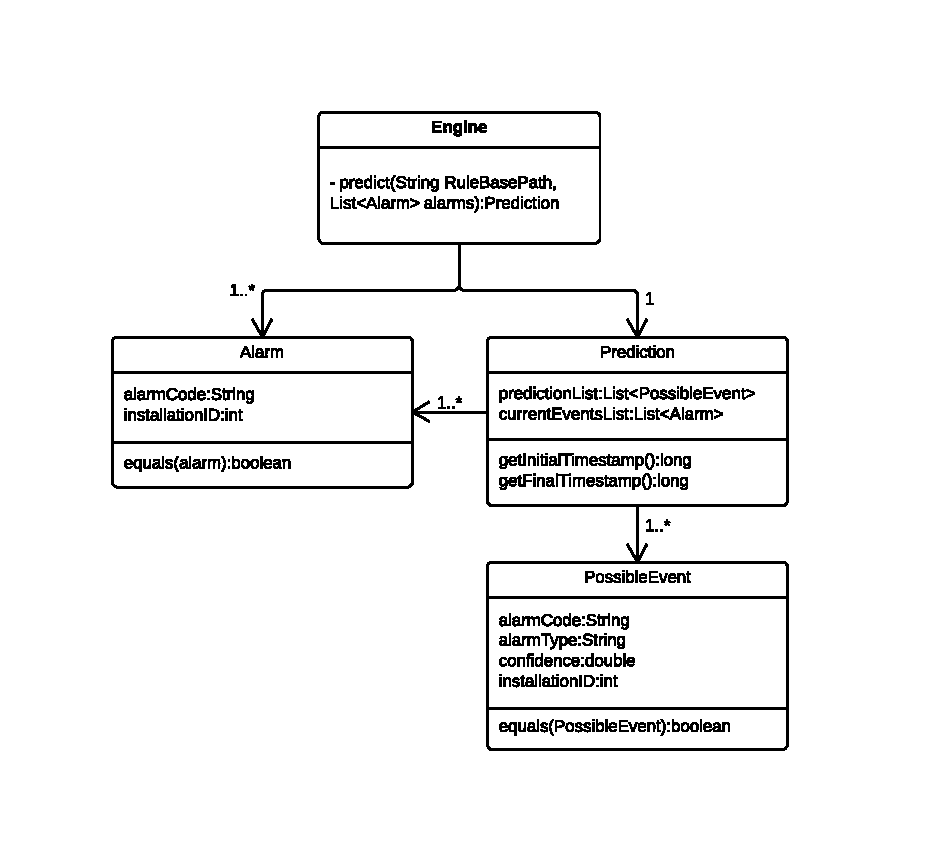
\includegraphics[width=\textwidth]{img/prototypeArchitecture.pdf}
\caption{Class diagram for the implemented module} \label{fig:prototypeArchitecture}
\end{figure}

\subsection{Input selection and execution}
As described in section~\ref{sec:parameters_and_interfaces}, our module takes a list of Alarm objects and outputs a Prediction object containing a list of PossibleEvent objects. We have also seen that it is important to provide an input which adequates to the conditions imposed by the selected rule set (or viceversa), which simply means that we must provide a list containing an observation time whose length adequates to that expected by the rule set.

Furthermore, as seen in figure~\ref{fig:prototypeArchitecture}, Alarms are described not only by their alarm code, but also by the installation in which they have been raised. It is important to have into account that alarms are only related to others happening in the same installation, and therefore we only need inputs to contain sets which are complete in terms of installation id. In other words, we could call the inference engine with separated inputs containing each the alarms which have been raised by each of the installations. However, as the rule sets are the same for all of the installations under the same maintenance station, it is more efficient to make this distinction during execution instead of having to call the engine and load the rules several times.

\subsection{The rule engine}
In section~\ref{sec:module_description} we introduced the concept of \emph{the rule engine}, the core of our module in which most of the heavy processing happens. Amongst all the available solutions, we selected the \emph{Drools Expert}\cite{browne2009jboss} platform, as it is the most advanced solution available for Java environments, and therefore an easy integration can be made with the rest of the maintenance station software.

\emph{Drools Expert} relies on \emph{Drools rule files}, which are plain text files containing our rules coded with an special syntax. Furthermore, it provides several ways of managing and even changing these rules, as interfaces for business users or other tools to easily generate these files based on workflow diagrams or other sources. However, as the knowledge on which our rules are based is obtained from a different source (a fully independent Data Mining process) we won't make use of these posibilities and will just have to consider the output format for our rules, to make it directly compatible with Drools' syntax. In section~\ref{sec:description_of_rule_sets} we will provide further description of these rule sets, as well as their generation and conversion processes.

Our module encapsulates and streamlines the execution of Drools Expert and their preparation process. The details of this configuration are of little relevance, and can be summarized as \emph{choosing a rule set} and \emph{provide a valid input}. Our module will then simply evaluate all the rules and then provide an output with a prediction for the next period, as we described in section~\ref{sec:parameters_and_interfaces}. The cornerstone of all this process is therefore the rule set. As we will describe in section~\ref{sec:description_of_rule_sets}, it is of essential importance to carefully build these in order to obtain a proper function of the rule engine. In the end, the rules are actually part of the code of our module, on which reiles most of its functionality.

A sequence diagram of the module's function can be seen in figure~\ref{fig:prototypeSequence}

\begin{figure}[hbtp]
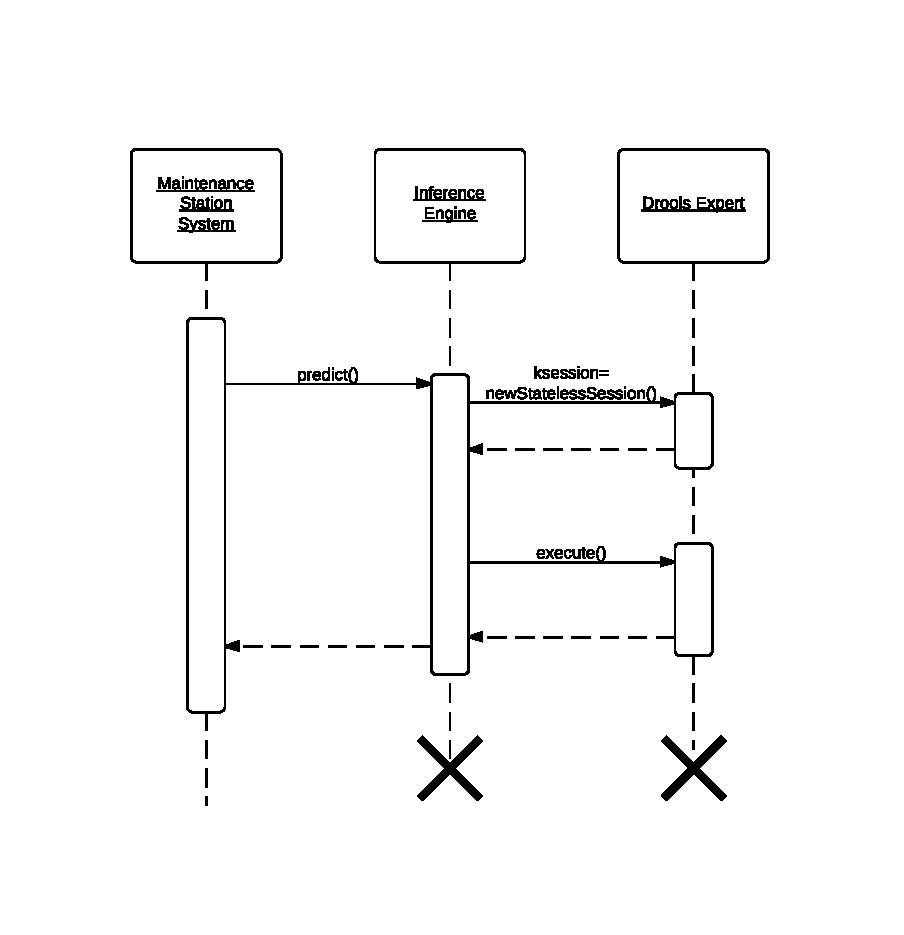
\includegraphics[width=\textwidth]{img/prototypeSequence.pdf}
\caption{Sequence diagram for the implemented module} \label{fig:prototypeSequence}
\end{figure}

\section{Description of rule sets}
\label{sec:description_of_rule_sets}
In this section we are going to describe the most important part of our prediction module: the rule sets. A rule set is simply a plain text file containing the necessary information for a rule to be evaluated and fired in the adequate circumstances. A rule can be simply seen as a piece of information stating that "When \emph{A} and \emph{B} happen, \emph{C} will happen with a certainty of 80\%", but there is actually a few more compexity added for the proper functioning of our system.

First of all, as we mentioned in section~\ref{sec:parameters_and_interfaces}, we have to take into account that events have to happen in the same installation for alarms to be raised. In other words, the rule above would be actually needed to be stated as follows:

\emph{"When A happens, and B happens in the same installation as A, C will happen in the same installation with a certainty of 80\%"}

Also, although it is not necessary for the basic function of our module, we will also return the type of alarm we are predicting in the output. The type of alarm can be directly inferred from the alarm code itself, but as we are working with hardcoded rulesets which only need to be generated once, it is much more efficient to associate the alarm type with each rule than having to perform a search every time an event is predicted. This does not affect how or module works at all, but our rule will actually look more like:

\emph{"When A happens, and B happens in the same installation as A, C (Which is an event of type 1) will happen in the same installation with a certainty of 80\%"}

This information can be useful to provide an overview of the kind of systems which are more prone to fail in a short future, and probably assign resources to groups instead of actual specific events for organisational convenience.

It is important to note that we are not mentioning at all time periods either for the observation (events A and B) or the expectation (event C). As we mentioned in section~\ref{sec:parameters_and_interfaces}, those parameters are implicit to the whole set of rules. For example, we \emph{know} we are talking of an observation of one day and a prediction for one day in the future because we are loading the ruleset whose rules work with that time windows. This is much more convenient as reduces the complexity of the rules avoiding having to handle additional parameters, but needs that the calling process takes into account these parameters by itself.

The same applies for the type of station we are working with. Even though the stations we are working with are quite different from each other, we do not specify in the rules where do we expect those events to hapen. Or we don't specify that \emph{explicitly}, because again, each rule set works exclusively for one specific station.

There is also a third parameter which we can directly affect simply by selecting an specific rule set: confidence. Instead of having to filter rules by their confidence when setting a threshold, it is much more efficient and convenient to load only those rules which provide predicitons with a confidence higher than a given threshold. As we mentioned, rulesets are plain text files which contain all the rules to be loaded, so by simply removing those with low confidence, we can perform this filtering in a very efficient way.

It is up to the maintenance operator to decide upon these thresholds. In order to be on the safe side, we usually set a threshold of 50\% (which is, predictions which are more likely to be right than wrong), but for an operator it might be more convenient to disregard maybe even predictions whose confidence are lower than 70\% or 80\%. By directly removing those rules from the rule sets, the additional computation needed to evaluate them is eliminated, and therefore the execution would be much more efficient.

The specific list of sets which have been generated and provided can be seen in table~\ref{tab:ruleset_list}.

\begin{table}
\begin{center}
\begin{tabular}{|c|c|c|c|c|}
\hline \headcell{Rule set} & \headcell{Station} & \headcell{Observation} & \headcell{Prediction} & \headcell{Min. Confidence} \\ 
\hline 
albacete1d\_70.drl & Station A & 1 day & next day & 70\% \\ 
\hline  
albacete7d\_70.drl & Station A & 7 days & next 7 days & 70\% \\ 
\hline 
antequera1d\_70.drl & Station B & 1 day & next day & 70\% \\ 
\hline 
segovia1d\_70.drl & Station C & 1 day & next day & 70\% \\ 
\hline
segovia2d\_70.drl & Station C & 2 days & next 2 days & 70\% \\  
\hline 
segovia7d\_70.drl & Station C & 7 days & next 7 days & 70\% \\  
\hline 
sevilla1d\_70.drl & Station D & 1 day & next day & 70\% \\ 
\hline
albacete1d\_50.drl & Station A & 1 day & next day & 50\% \\ 
\hline 
albacete7d\_50.drl & Station A & 7 days & next 7 days & 50\% \\ 
\hline 
antequera1d\_50.drl & Station B & 1 day & next day & 50\% \\ 
\hline 
segovia1d\_50.drl & Station C & 1 day & next day & 50\% \\ 
\hline
segovia2d\_50.drl & Station C & 2 days & next 2 days & 50\% \\  
\hline 
segovia7d\_50.drl & Station C & 7 days & next 7 days & 50\% \\  
\hline 
sevilla1d\_50.drl & Station D & 1 day & next day & 50\% \\ 
\hline
albacete1d\_all.drl & Station A & 1 day & next day & -- \\ 
\hline  
albacete7d\_all.drl & Station A & 7 days & next 7 days & -- \\ 
\hline 
antequera1d\_all.drl & Station B & 1 day & next day & -- \\ 
\hline 
segovia1d\_all.drl & Station C & 1 day & next day & -- \\ 
\hline
segovia2d\_all.drl & Station C & 2 days & next 2 days & -- \\  
\hline 
segovia7d\_all.drl & Station C & 7 days & next 7 days & -- \\  
\hline 
sevilla1d\_all.drl & Station D & 1 day & next day & -- \\ 
\hline

\end{tabular} 
\caption{Generated rule sets} \label{tab:ruleset_list}
\end{center}
\end{table}

\subsection{Generation of rule sets}
\label{sec:generation_of_rule_sets}

We have mentioned in section~\ref{sec:module_description} that our rules are obtained through a \emph{Data Mining process}, and later translated into the Drools syntax. In this section we are going to give an overview of the whole process.

Everything starts with a database backup provided by Thales' engineers which contains a large amount of event logs in all the stations we are going to study. That database is transformed into a working set, a process which involves several processes such as variable reduction, data normalisation and format conversion. This data is loaded into an R\cite{ihaka1996r, torgo2003data} environment in which the core data mining procedure is performed: the rule discovery process. This step forms the core of the whole procedure, and requires a considerable amount of resources and time.

This generates a raw list of association rules, in the format of R data frames. At this point we can already perform some filtering to separate the useful rules from those with very low confidence values. However, as those rules can also be useful for future research or to be manually analysed by maintenance operators, so far we have decided to save the whole amount of generated rules whichever their precision was.

A last process is performed in which we convert the raw R data frames\cite{ihaka1996r} containing the rules into the Drools syntax. At this point we also generate several subsets with different confidence thresholds, as mentioned in section~\ref{sec:description_of_rule_sets}. This step is fully automated with Python\cite{sanner1999python} scripts. An example of both formats will be shown in section~\ref{sec:structure_of_rules_and_sets}.

A diagram of the whole process can be seen in figure~\ref{fig:prototypeGenProcess}.

\begin{figure}[hbtp]
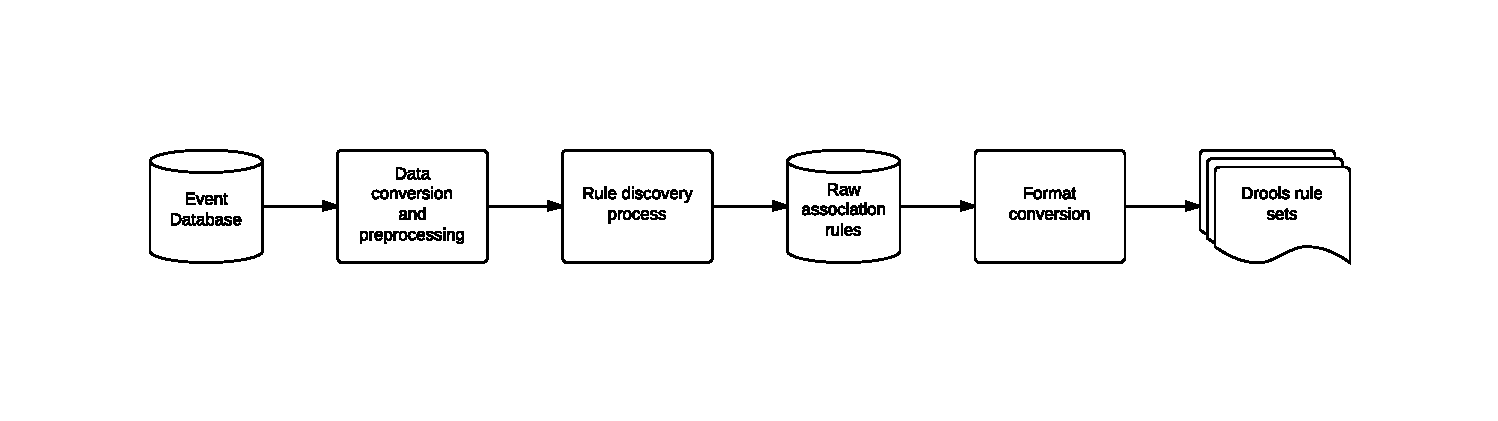
\includegraphics[width=\textwidth]{img/prototypeGenProcess.pdf}
\caption{The whole rule generation process} \label{fig:prototypeGenProcess}
\end{figure}

\subsection{Structure of rules and sets}
\label{sec:structure_of_rules_and_sets}
In this section we will now analyse the actual structure of our rules and their conversion to the Drools syntax. We will take the following rule as an illustrating example:

\begin{framed}
\begin{lstlisting}[style=mono]
"<{
	saml.status.energy_net1_not_present
	saml.status.energy_net2_not_present
	saml.status.energy_48V_battery_nok
	saml.status.energy_SAI_PT_nok
},{
	saml.status.energy_SAI_ST_nok
}>",
0.83833333,
0.089034423
\end{lstlisting}
\end{framed}

That is the appearance of a prediction rule in the format of R data frame. Lines 2, 3 and 4 are the antecedents, line 6 is the predicted event and rule 8 is the precision of the rule. The last number on line 9 is the recall of the rule, an evaluation value which is of no use at this moment.

The same rule in Drools syntax would looks as follows:

\begin{framed}
\begin{lstlisting}[style=mono]
rule "rule0"
    when 
        Alarm(iid : installationID, alarmCode 
        		== "saml.status.energy_net1_not_present");
        Alarm(installationID == iid, alarmCode 
        		== "saml.status.energy_net2_not_present");
        Alarm(installationID == iid, alarmCode 
        		== "saml.status.energy_48V_battery_nok");
        Alarm(installationID == iid, alarmCode 
        		== "saml.status.energy_SAI_PT_nok");
    then 
        PossibleEvent p = new 
        	PossibleEvent("saml.status.energy_SAI_ST_nok",
        			"fieldElementFailure",iid,0.83833333);
        resultList.add(p);
end
\end{lstlisting}
\end{framed}

We can see here the additions mentioned in section~\ref{sec:description_of_rule_sets}, regarding installation code and event type (which is hardcoded here to "filedElementFailure"). The resultList object conforms the output which will be returned by Drools to our module, containing all the generated possible events.

\section{Output visualisation}
When describing our predictive module, we haven't so far spoken on how this data is visualised or shown to maintenance operators. This is because our module does not provide a visual interface in any way to make this data user-readable. The predictive module is meant to be integrated in a much larger system which is Thales' railway maintenance station software. This will provide operators a visualization of the predictions, and can even provide means for automatic prediction handling.

However, in order to illustrate the possibilities offered by the implemented prototype, we have developed a demonstration interface. This illustrative example can be seen in figure~\ref{fig:demoExample}.

\begin{figure}[hbtp]
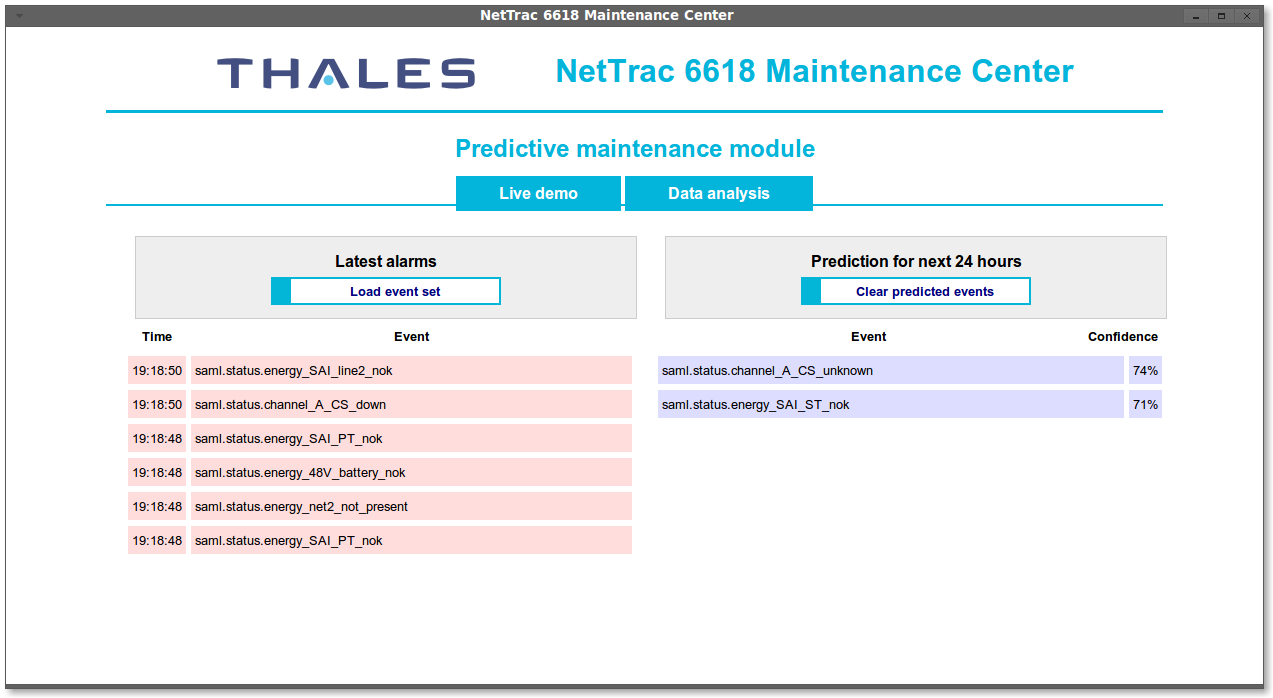
\includegraphics[width=\textwidth]{img/demoExample.png}
\caption{Example demo interface} \label{fig:demoExample}
\end{figure}

\clearpage

\section{Conclusions}
At this stage of the project, we have already developed a fully functional predictive module to be integrated within Thales' maintenance station. Furthermore, a demo interface has been provided in order to illustrate one of the multiples applications this module can offer to maintenance operators.

However, the module allows Thales' engineers to perform much more advanced tasks with these predictive information. From statistical reports including information on the predictions, to automatic processes started as response to specific predicted events, the range of possibilities is quite large.

Integration is also possible within any other kind of system, due to the implementation of the module as a Java library. Furthermore, it is even possible to build a standalone predictive system, performing predictions sobre already generated static event sets.

In general terms, the implementation of the module has been successful and completely fulfils our goals.

\clearpage
